% Created 2021-12-17 Fri 08:44
\documentclass[9pt, b5paper]{article}
\usepackage[UTF8]{ctex}
\usepackage{xltxtra}
\usepackage{bera}
\usepackage[T1]{fontenc}
\usepackage[scaled]{beraserif}
\usepackage[scaled]{berasans}
\usepackage[scaled]{beramono}
\usepackage{graphicx}
\usepackage{xcolor}
\usepackage{multirow}
\usepackage{multicol}
\usepackage{float}
\usepackage{textcomp}
\usepackage{geometry}
\geometry{left=1.2cm,right=1.2cm,top=1.5cm,bottom=1.2cm}
\usepackage{algorithm}
\usepackage{algorithmic}
\usepackage{latexsym}
\usepackage{natbib}
\usepackage{minted}
\newminted{common-lisp}{fontsize=ootnotesize}
\usepackage[xetex,colorlinks=true,CJKbookmarks=true,linkcolor=blue,urlcolor=blue,menucolor=blue]{hyperref}
\author{deepwaterooo}
\date{\today}
\title{Android Study Plan}
\hypersetup{
  pdfkeywords={},
  pdfsubject={},
  pdfcreator={Emacs 27.1 (Org mode 8.2.7c)}}
\begin{document}

\maketitle
\tableofcontents


\section{Daily updates}
\label{sec-1}
\begin{itemize}
\item 因为需要准备一个面试,这几天不更新算法系列,只准备安卓面试
\item win 10 wsl 1 ubuntu 18 adb configuration done, not complicated, once search for solutions, and config, it works.
\item api levle 30 androidx basic project environment can be configured, but dynamic fragment add not done yet, switched back to api 28 temporatorily
\item wsl 1 ubuntu 18 adb logcat is so slow. after 9pm yesterday, 150K lines of log, I could only adb logcat previous project samplefragments, can can not grab any FirstFragment nor Second Fragment Log.i info. may switch laptop back to Mac, but it has only 8GB memory, and internet too slow for that laptop
\item today will review major components, as well small details, notes summaries to move on
\item \textbf{恶鬼们昨天晚上今天早上又疯狂作案一晚,一个故意晚回来,用洗手间,用厨房,半夜一两点钟还在故意厨房里开厨导柜吵别人;一个今天早上五点钟便受恶房东暗示指使,故意开车库噪音极大的声响,早上五点钟便故意吵醒别人休息,实在是无恶不作(它有昨天晚上下班后到休息前一晚上的时间他不提前装车,非要等到早上五点钟故意把别人吵醒,另一个贱畜牲的做法是在别人晚上入睡前故意吵别人,贱蓄牲们的做法还不够猖狂吗?)}
\item BroadcastReceiver sample project runs though easily. Will look into ContentProvider projects too today, all of them are not complicated.
\item ContentProvider Interprocess communication projects are connected well too. One functions as server, the other as client, not complicated at all.
\end{itemize}

\section{Adidev Technology, Inc 围堵封杀职场女性职业生涯细节记}
\label{sec-2}
\begin{itemize}
\item 对一个职场女性的围堵与封杀,何时为了?
\end{itemize}

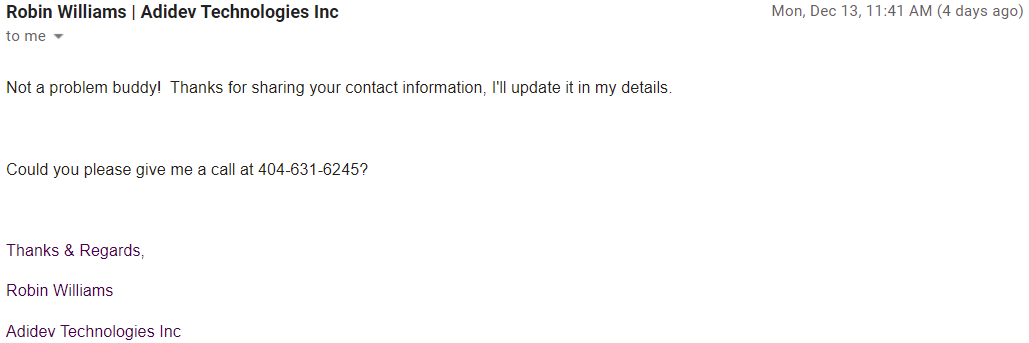
\includegraphics[width=.9\linewidth]{./pic/buddy.png}

\begin{itemize}
\item 围堵? 故意下套碰磁?这个等今天下午的时候,或傍晚的时候再回来写
\end{itemize}

\section{系统服务篇}
\label{sec-3}
:clock1: DONE: Android 如何启动?
[x] DONE: Android 应用进程启动流程
[ ] 什么是系统服务?
[ ] ActivityManagerService
[ ] SystemServer
[x] DONE: Android 应用安装过程源码解析
[ ] WindowManagerService
[ ] Zoyote 前世今生

\section{通信框架篇}
\label{sec-4}
[x] Binder 完全解析
[x] DONE: Binder 完全解析(一)概述
[x] DONE: Binder 完全解析(二)设计详解
[x] DONE: Binder 完全解析(三)AIDL实现原理分析
[x] Handler 通信框架
[x] DONE: Handler消息机制源码解析

\section{应用组件篇}
\label{sec-5}
[ ] Application 是什么?
DONE: Context 分析
[ ] Activity 组件分析
[x] DONE: Activity生命周期是如何实现的
[ ] Services 组件分析
[ ] ContentProvider 组件分析
[ ] Broadcast 组件分析

\section{珠玑拾遗}
\label{sec-6}
[ ] Gradle 用法
[ ] 混淆一二事

Andriod系统开发

\section{Android操作系统概述}
\label{sec-7}
Android平台介绍;Android平台特性;Android平台架构;Android Navtive C/C++程序开发;Android NDK;Native开发方式与JAVA开发方式比较。
\section{Android开发环境搭建}
\label{sec-8}
Android SDK介绍;Eclipse ADT插件;Android模拟器开发。
\section{Android项目结构分析}
\label{sec-9}
资源管理(Resources)分析;drawable分析;layout分析;Activity分析;Intent分析;Service分析;Content分析。
\section{Android UI设计}
\label{sec-10}
标准控件的使用;设计开发自定义控件;Layout布局的使用;触摸/按键(UI Events)事件处理方法;View,SurfaceView,Canvas,Paint类分析使用;显示文本以及显示特殊效果文本;绘图及显示图片;实现动画效果。
\section{Intent Receive}
\label{sec-11}
Intent的作用和目的;属性讲解;Android定义解析Intent;AndroidManifest.xml深入分析。
\section{Service}
\label{sec-12}
什么是Service,如何使用Service,Service的生命周期,BroadcastReceiver的使用。
\section{Content Provider}
\label{sec-13}
SQLite介绍,创建Content Providers,使用Content Providers,使用URI语法进行增删改查。
\section{Android高级应用开发}
\label{sec-14}
访问本地通讯录;网络连接的相关知识;流媒体的处理;URLConnection和HttpURLConnection的应用;
HttpClient的分析;本地文件浏览管理;音视频播放处理;Widget应用开发。
\section{Android程序发布部署建}
\label{sec-15}
Android 调试桥;启用logcat日志调试;模拟器上安装删除软件;打包* 签名和安装软件到设备。
\section{Android 底层架构分析}
\label{sec-16}
移植Android到新的硬件平台;需要支持Linux 操作系统的硬件平台架构分析;支持Android的Linux内核特性分析;为Linux内核增加Android特性;移植Android Debug Bridge调试接口;编写/移植Android内核驱动;硬件支持double frame buffer/page flipping;bionic库移植与优化;Dalvik Vm移植;第三方应用程序移植;建立Android移植开发平台;新的嵌入式处理器引入的Android相关问题;获得高效的Android工具链。
\section{Android移植}
\label{sec-17}
支持ARM11的Linux-2.6.28内核新特性简介;移植LCD double buffer驱动;移植触摸屏驱动;移植Android键盘驱动;移植Wifi驱动支持Android上网功能;移植电源管理驱动,支持Android电池管理;部署Android系统到实际ARM11平台。
\section{阶段项目实战与测试}
\label{sec-18}
通过对ITelephony接口和ISms接口以及AIDL在Android程序中的开发应用,开发一个打电话和发短信的程序。

\section{自定义view Android 11 api level android M}
\label{sec-19}
\subsection{gradle.properties}
\label{sec-19-1}
\begin{minted}[frame=lines,fontsize=\scriptsize,linenos=false]{xm}
android.useAndroidX=true
landroid.enableJetifier=true
\end{minted}
\begin{itemize}
\item 什么是Jetifier? 例如,要使用androidx打包的依赖项创建新项目,此新项目需要在gradle.properties文件中添加以下行:
\end{itemize}

java version 8
 compileOptions \{
        sourceCompatibility JavaVersion.VERSION$_{\text{1}}$$_{\text{8}}$
        targetCompatibility JavaVersion.VERSION$_{\text{1}}$$_{\text{8}}$
    \}

import android.os.Bundle;
import android.support.design.widget.FloatingActionButton;
import android.support.design.widget.Snackbar;
import android.view.View;
import android.view.Menu;
import android.view.MenuItem;
import androidx.appcompat.app.AppCompatActivity;
import androidx.appcompat.widget.Toolbar;
import com.google.android.material.floatingactionbutton.FloatingActionButton;
import com.google.android.material.snackbar.Snackbar;

<com.me.generalprac.CustomTitleView
    android:layout$_{\text{width}}$="match$_{\text{parent}}$"
    android:layout$_{\text{height}}$="wrap$_{\text{content}}$"/>
<include layout="@layout/custom$_{\text{title}}$"/>

\section{Good morning Robin,}
\label{sec-20}

Among all my previous interviews and coding tests, I have always been sharing my screen with interviewer so that interviewee (like me) can coding at his/their most confortable working/coding environment. 

This may sound different from your intuition, as we all understand that staffing company tries their best to decrease salaries of their employee so that they the company can benefit more from the client company pay rate difference to the employee. And this could be the most significant reason you guys -- staffing companies try all your best to limit the candidates from performing their best. 

I stated above only because I am an Emacs geek, and I started using command line based editor emacs ever since the first day of my programming career (my github account: \url{https://github.com/deepwaterooo?tab=repositories} . It even has the emacs repository). 

I REFUSE such unreasonable test (I had never have any such wired requirments, and this is the reason I am writing to you to negociate possible better solutions). But if you consider sharing screen so that Adidev can monitor my coding process through sharing screen, through my emacs editor (you can monitor my coding process through my emacs editor and I would paste final result into your coding link too, so that you can still score or evaluate using your test system framework.)

Please do help consider sharing screen instead of limiting the candidate's performance at your best effort. If you don't consider such options, I refuse such unreasonable tests, only because I am a emacs geek, and I am not interested in such wired coding test. 

Please let me know if you have any question, or opinions. 

thanks, and regards 
% Emacs 27.1 (Org mode 8.2.7c)
\end{document}